%%%%%%%%%%%%%%%%%%%%%%%%%%%%%%%%%%%%%%%%%%%%%%%%%%%%%%%%%%
%% HEIG-VD
%%
%% Modèle Latex pour laboratoire de POO
%% Basé sur le chablon de CSN crée par MiM
%% 
%% Fichiers à changer : 
%%            - constantes.tex
%%            - Tous les fichiers du corps du rapport 
%%
%% Auteur : Emily Baquerizo
%% Date   : 06.10.24
%%%%%%%%%%%%%%%%%%%%%%%%%%%%%%%%%%%%%%%%%%%%%%%%%%%%%%%%%%

% Paramétrage du papier utilisé
\documentclass[a4paper,12pt,oneside]{article}

% Ne pas toucher, nécessaire à la mise en forme
\usepackage[utf8]{inputenc} 
\usepackage[T1]{fontenc} % Nouvelle norme pour codage des caractères
\usepackage{lmodern} % Nouvelle forme de la fonte ComputerModern
\usepackage{babel} % Règles typographiques françaises, césures
\babelprovide[import, main]{french}
\usepackage{graphicx} % Insertion images
\usepackage{epstopdf} % Convertir les images eps vers pdf
\epstopdfsetup{outdir=./Images/converted\_to\_pdf/} % Dossier de sortie des images converties
\pagenumbering{arabic}
\usepackage[top=3cm, bottom=3cm, left=3cm, right=3cm, showframe=false]{geometry}
\usepackage{amsmath}
\usepackage{hyperref}
\usepackage{pdfpages}
\usepackage{color}
\usepackage{titlesec} % Indente les sous-sections pour améliorer la visibilité
\usepackage{float} % Pour forcer la mise en place de l'image

% fichier avec les constantes(étudiants, prof, labo, etc) A ADAPTER POUR CHAQUE LABO
%%%%%%%  Constantes (à changer) %%%%%%%%

\newcommand{\nomAuteur}{Emily Baquerizo \& Kimberly Beyeler}

\newcommand{\titre}{AI and Vision-based navigation}

\newcommand{\nbrlabo}{02} % numéro de laboratoire

\newcommand{\prof}{Marina Zapater}

\newcommand{\assistant}{Guillaume Chacun \& Mehdi Akeddar}

\newcommand{\classe}{IAA-A}

\newcommand{\departement}{Technologies de l'Information et de la Communication (TIC)}

\newcommand{\cours}{Intelligence Artificielle pour les Système Autonomes (IAA)}

\newcommand{\dateRendu}{15 avril 2026}

% Entête et pieds de page (A ADAPTER)
\pagestyle{empty}
\usepackage{fancyhdr}
\setlength{\headheight}{27.06pt}
\pagestyle{fancy}
% Entête :
\renewcommand{\headrulewidth}{1pt}
\fancyhead[L]{Labo \nbrlabo: \titre} 
\fancyhead[R]{Rapport de laboratoire} 
% Pied de page
\fancyfoot{} % clear all footer fields
\renewcommand{\footrulewidth}{1pt}
\fancyfoot[R]{Page \thepage} 
\fancyfoot[L]{HEIG-VD | \nomAuteur }

% Package formatage de code C
\usepackage{listings}
\usepackage{xcolor}

% Package tableau
\usepackage{tabularx}


\lstset{
  language=C,
  basicstyle=\ttfamily\small,
  numbers=left,
  numberstyle=\tiny\color{gray},
  keywordstyle=\color{blue}\bfseries,
  commentstyle=\color{gray}\itshape,
  stringstyle=\color{orange},
  frame=single,
  tabsize=4,
  showstringspaces=false,
  breaklines=true
}

% debut du corps du rapport 
\begin{document}	
	% première page
	%%%%%%%%%%%%%%%%%%%%%%%%%%%%%%%%%%%%%%%%%%%%%%%%%%%%%%%%
% Ce document ne doit pas être modifié
% Il faut modifier les informations depuis le fichier
% constantes.tex
%%%%%%%%%%%%%%%%%%%%%%%%%%%%%%%%%%%%%%%%%%%%%%%%%%%%%%%%



\begin{flushleft}
	
\includegraphics[height=2cm]{./images/logo_heig.pdf}
\end{flushleft}

\vfill

\begin{center}
	\Large Laboratoire \nbrlabo:\\
	\huge \titre \\
\end{center}


\begin{center}
	\begin{tabular}{l l}
		Département:          & \departement\\
		Unité d'enseignement: & \cours\\
	\end{tabular}
\end{center}


\vfill

%\begin{center}
%	\includegraphics{Images/it.png}
%\end{center}

\vfill

\begin{tabular}{l l}
	\Large	Autrices:   	  & \Large \nomAuteur\\
	Professeure:           & \prof\\
	Assistants:			  & \assistant\\
	Classe:               & \classe\\
	Date:                 & \dateRendu\\
\end{tabular}

\vfill

\begin{center}
\hfill 
\includegraphics[height=2cm]{./images/logo_hesso.pdf}
\end{center}
	% enlève le numero sur la premiere page
	\thispagestyle{empty}
	\setcounter{page}{1}
	\newpage
	
	% ici débute le corps du rapport
	% changer les sections au cas par cas afin de vous adapter au maximum aux critères
	% Table des matières
	\tableofcontents
	\newpage % Commence une nouvelle page
	%\section{Introduction}
	%\input{chapitres/Introduction.tex}
	%\section{Partie 1}
	\section{Dataset study}
on essaie promis
	%\section{Partie 2}
	\section{Choix du modèle}
\subsection{Architecture}
Le modèle choisi est ResNet18 pré-entraîné sur ImageNet et se nomme DuckieNet. Nous avons fait ce choix pour plusieurs raisons : 
\begin{itemize}
  \item Taille compacte : ResNet18 compte 11.7M paramètres, ce qui est un bon compromis entre capacité d'apprentissage et vitesse d'inférence sur le Jetson Nano embarqué du Duckiebot.
  \item Apprentissage par transfert : les features extraites des premières couches (textures, contours, formes) sont directement réutilisables pour la reconnaissance de routes, sans nécessiter un entraînement from scratch coûteux.
  \item Architecture des couches : ResNet18 est composé de 4 blocs résiduels (layer1 à layer4), chacun avec 2 blocs de convolutions. La tête de classification originale est remplacée par une tête de régression personnalisée : \texttt{Linear(512 → 128) → ReLU → Dropout(0.3) → Linear(128 → 2)}. La sortie est un vecteur de 2 valeurs : \texttt{[vel_left, vel_right]}.
  \item Stratégie de gel des couches : lors de l'entraînement initial, seuls layer4 et fc sont entraînés, les couches précédentes restant gelées. Cela accélère l'entraînement et évite le sur-apprentissage sur le dataset synthétique. La même stratégie est appliquée lors du fine-tuning.
\end{itemize} 
\subsection{Paramètres d'entraînement}
L'entraînement initial est effectué sur 20 epochs avec un batch size de 32 et un learning rate de 1e-3. Le fine-tuning est effectué jusqu'à convergence des courbes de loss, avec un arrêt manuel basé sur l'observation du plateau de la val loss, en utilisant un batch size de 16 et un learning rate de 1e-5. \\
Dans les deux cas, l'optimiseur Adam est utilisé pour sa convergence rapide et sa gestion automatique du learning rate par paramètre. La fonction de perte choisie est la MSELoss, adaptée à la nature continue de la tâche de régression. Le scheduler ReduceLROnPlateau réduit le learning rate d'un facteur 0.5 lorsque la val loss stagne, avec une patience de 3 epochs pour l'entraînement initial et 2 epochs pour le fine-tuning, évitant ainsi de rester bloqué dans un minimum local.
\subsection{Fine-tuning}
Le modèle entraîné sur le dataset synthétique présente un domain gap avec les images réelles du robot qui mène à des sorties de circuit lors du déploiement.
Pour y remédier, un fine-tuning est effectué sur le dataset réel collecté manuellement. Plusieurs choix ont été faits :
\begin{itemize}
  \item Chargement depuis le meilleur checkpoint : le fine-tuning repart de best_model.pt via init_and_load, garantissant que les poids de départ sont optimaux.
  \item Gel partiel conservé : seuls layer4 (dernier bloc convolutif de ResNet-18) et fully connected restent entraînables, les couches basses étant gelées. Avec 7 198 échantillons réels, entraîner toutes les couches risquerait de causer un overfitting et d'effacer les features générales apprises sur ImageNet.
  \item Learning rate réduit : le passage de 1e-3 à 1e-5 permet des mises à jour douces qui adaptent le modèle sans détruire les connaissances acquises. 
  \item Split aléatoire : le dataset réel est divisé aléatoirement en 80\% train et 20\% val via train_test_split, évitant le biais d'un split séquentiel qui aurait pu concentrer les virages dans un seul split.
\end{itemize}

	%\section{Partie 3}
	\section{Global Performance}
\subsection{Global Performance}
L'entraînement initial sur le dataset synthétique donne les résultats suivants à convergence : 
\begin{itemize}
    \item MSE Loss : 0.0006 (entraînement et validation)
    \item MAE : 0.016 (entraînement et validation)
\end{itemize}
Les courbes montrent une convergence rapide en 2-3 epochs sans overfitting. 
La val loss légèrement inférieure à la train loss confirme que le dataset 
synthétique est homogène et peu varié. \\

\subsection{Fine-tuning (dataset réel)}
Le fine-tuning sur le dataset réel donne les résultats suivants à convergence :
\begin{itemize}
    \item MSE Loss : 0.017 (validation)
    \item MAE : 0.098 (validation)
\end{itemize}
Les courbes de train et validation descendent conjointement sans divergence, 
indiquant une bonne généralisation sans overfitting. 

\subsection{Analyse comparative}
La MAE est environ 6 fois plus élevée après fine-tuning sur données réelles 
(0.098) qu'après entraînement sur données synthétiques (0.016). 
Cette différence s'explique par la plus grande variabilité des données réelles : 
bruit, variations d'éclairage et calibration spécifique du robot.

Cependant, les métriques numériques ne sont pas le seul critère de succès. 
Le vrai test est le comportement du robot sur piste : le modèle entraîné 
uniquement sur données synthétiques sortait régulièrement du circuit, 
tandis que le fine-tuning vise à corriger ce comportement en adaptant 
le modèle à la réalité physique du robot. \\

\subsection{Tests sur le robot}
Par manque de temps, nous n'avons pas pu tester le modèle final sur le robot.

	%\section{Partie 4}
	\input{chapitres/Partie_4.tex}
	%\section{Issues}
	\section{Issues Encountered}

Lors de ce laboratoire, nous avons rencontré de nombreux problèmes. Lors de la mise en place du projet, nous avons constaté que seul un des deux ordinateurs du groupe pouvait se connecter au robot et ce, malgré de nombreuses tentatives.

Nous avons également appris à nos dépens qu'il ne fallait pas retirer la carte SD pendant que le robot était allumé, nous offrant ainsi, un casse-tête à tenter de réparer le robot pendant toute une semaine. 

Après avoir réglé tout cela, nous nous sommes heurtées à un nouveau problèmes lors de la data collection manuelle. Nous avons constaté que le robot ne réagissait pas de la manière désirée selon les touches appuyées.
	%\section{Partie 5}
	%\input{chapitres/Partie_5.tex}
	%\section{Partie 6}
	%\section{6ème partie : Réparation}

\subsection{Manipulation 8.1}
\textbf{En utilisant les programmes que vous avez codés, déchiffrez tous les documents fournis dans le dossier \texttt{/home}.}\newline

Les trois fichiers n'ont pas été lisibles après plusieurs tentatives de déchiffrement, nous obtenons du "bruit" à la place du texte clair, un détail nous échappe forcément lors de notre analyse des fonctions de chiffrement. 

\subsection{Question 8.1}
\textbf{Expliquez l'algorithme de déchiffrement que vous avez implémenté. Indiquez les formules mathématiques appliquées par chaque méthode de déchiffrement ainsi que la logique du flux d'instruction qui permet d'appliquer l'une ou l'autre.}\newline

\begin{itemize}
\item \textbf{Choix de la méthode } : calculer
\[
\text{mode} \;=\; \big(\text{char\_occurrences}(\text{filename})\big)\ \&\ 3
\]
puis appliquer
\[
\begin{cases}
\text{decrypt0} & \text{si }\text{mode}=0,\\
\text{decrypt1} & \text{si }\text{mode}=1,\\
\text{decrypt2} & \text{si }\text{mode}=2.
\end{cases}
\]

\item \textbf{decrypt0 (inverse de \texttt{encrypt0})} : pour chaque byte lu \(c\) on applique un XOR conditionnel :
\[
K=\begin{cases}
0xEF &\text{si }(c\ \&\ 0x02)=0,\\[4pt]
0xBE &\text{sinon},
\end{cases}
\qquad
o \;=\; c \oplus K.
\]
Remarque : \( \oplus \) est son inverse, donc on applique la même opération et cela restaure l'octet original.

\item \textbf{decrypt1 (inverse de \texttt{encrypt1})} : notations : \(c\) octet chiffré, \(p\) valeur \texttt{char\_prev} (octet), \(o\) octet original.
\[
\text{(chiffrement)}\quad c = \big(\operatorname{ROL}_2(o)\; +\; p\big)\bmod 256
\]
\[
\text{(mise à jour)}\quad p \leftarrow (c\gg 2)\;|\;(c\times '@') \quad(\text{opération sur octet})
\]
Déchiffrement (l'ordre importe) : connaissant \(c\) et \(p\),
\[
r \;=\; (c - p)\bmod 256,\qquad o \;=\; \operatorname{ROR}_2(r),
\]
puis mettre à jour \(p\) exactement comme en chiffrement :
\[
p \leftarrow (c\gg 2)\;|\;(c\times '@').
\]

\item \textbf{decrypt2 (inverse de \texttt{encrypt2}) — deux passes} : soit \(N\) la longueur des données (taille fichier \(-1\)), et \(final\_temp\) l'octet final ajouter par \texttt{encrypt2}.

\begin{enumerate}
\item \textbf{Inverse de la 2\(^\text{ème}\) phase (XOR avec \(\text{temp}\) incrémenté)} : calculer l'état initial de \(\text{temp}\)
\[
\text{temp}_0 \;=\; \big(final\_temp - 4\cdot N\big)\bmod 256.
\]
Pour \(i=0\ldots N-1\) :
\[
A[i] \;=\; B[i] \oplus \text{temp},\qquad \text{temp}\leftarrow (\text{temp}+4)\bmod 256,
\]
où \(B[i]\) sont les octets présents (après première passe) et \(A[i]\) est la séquence reconstruite qui correspond à la sortie de la première passe.

\item \textbf{Reconstruire \(\text{key\_array1}\)} : appeler \(\texttt{generateKey}(\ldots)\) avec les mêmes paramètres constants que le binaire et découper la valeur 64-bits  comme dans \texttt{encrypt2} pour obtenir les bytes \(\text{key\_array1}[1\ldots 8]\).

\item \textbf{Inverse de la 1\(^\text{ère}\) phase} : initialiser \(\text{key\_index}=0\). Pour \(i=0\ldots N-1\) :
\[
\text{key\_index} \leftarrow (\text{key\_index}+5)\ \&\ 0xE,\qquad idx=\text{key\_index}+1,
\]
\[
o[i] \;=\; \big( (int8\_t)A[i] + (int8\_t)\,\text{key\_array1}[idx] \big)\bmod 256.
\]
Écrire \(o[i]\) sur la position \(i\).

\item \textbf{Tronquer} : supprimer le byte final en tronquant le fichier à longueur \(N\).
\end{enumerate}

\end{itemize}

\subsection{Manipulation 8.2}
\textbf{En utilisant ghidra, patchez le programme \texttt{calc} pour qu'il puisse à nouveau être utilisé sans risque.} \newline
Afin que le programme soit utilisé sans risque on va patcher en remplaçant le code assembleur : CALL \texttt{encrypt\_dir}

\begin{figure}[!htb]
	\centering
	\includegraphics[width=1\textwidth]{images/call}
	\caption{Instruction à patcher\\}
\end{figure}

Ensuite on fait : clique droit → patch instruction puis l'on remplace cette instruction par \texttt{NOP} sur 5 octets (Ghidra pourra générer 5 \texttt{NOP} consécutifs). Puis comme vu en cours, on peut valider le patch, Save (File → Save Program). Et enfin exporter le binaire patché (File → Export Program → ELF).





	%\section{Conclusion}
	%\input{chapitres/Conclusion.tex}
	%\section{Code}
	%%\appendix
%\section{Code}

%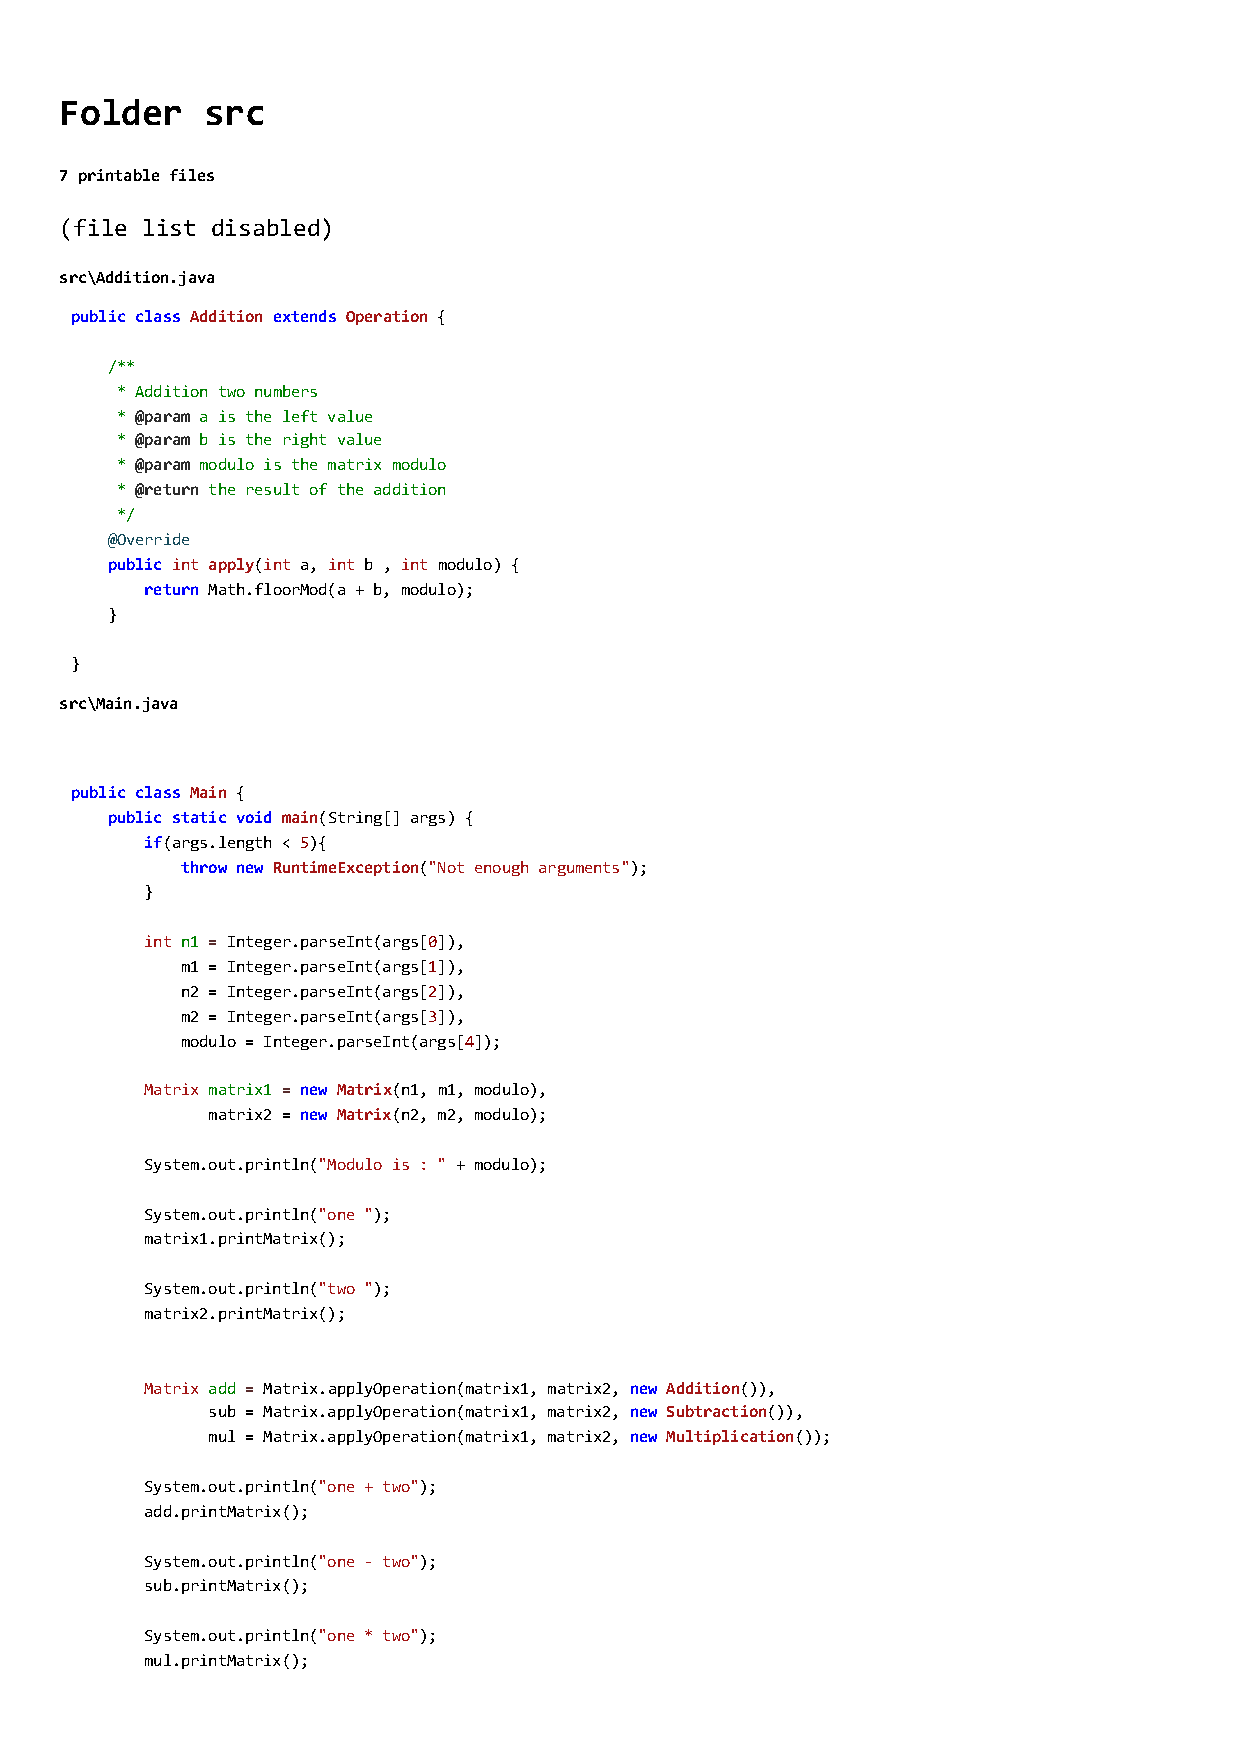
\includepdf[pages=-]{code/code.pdf}

	
	% si des annexes sont nécessaires ajouter : 
	% \section{Annexes}
	% Changement de notation en lettre : 
	%\appendix
	% insertion d'une nouvelle page
	%\newpage
	% Ajouter un fichier latec dans le fichier courant
	%\input{Chapitres/cdc.tex}
	
	%Fin du document
\end{document}


